\section{Materialización de los patrones: Patrones secundarios}

Si bien, como se definió en la sección \ref{sec_unidades}, el patrón primario de resistencia se basa en el Efecto Hall Cuántico por su inmutabilidad frente al tiempo, su implementación requiere condiciones de laboratorio extremas (criogenia y altos campos magnéticos). Para transferir esa exactitud a los laboratorios de calibración industrial y al uso cotidiano, se utilizan \emph{patrones secundarios} o de trabajo.

Estos son dispositivos físicos (resistores) diseñados para mantener un valor de resistencia lo más estable posible frente a variaciones ambientales (temperatura, humedad) y al paso del tiempo (envejecimiento).

\subsection{Arquitectura del patrón: La conexión Kelvin}

El método de medición a cuatro puntas, también conocido como método de Kelvin, es una técnica de medición de impedancia eléctrica que utiliza un voltímetro y un amperímetro para lograr mediciones más exactas de resistencia que al usar la técnica tradicional de medición a dos puntas. El método de medición a cuatro puntas es particularmente útil para la medición de resistencias pequeñas, ya que elimina las contribuciones de las resistencias de cableado y los potenciales de contacto sobre la medición final de la resistencia en cuestión; es por esto que algunos óhmetros de alta precisión se construyen utilizando circuitos similares.

Para resistores de bajo valor (típicamente \(R < \qty{10}{\ohm}\)), la resistencia de los propios cables de conexión y de los puntos de contacto puede ser comparable o superior al valor que se desea definir, introduciendo un error grosero inaceptable.

Para mitigar esto, los patrones de resistencia adoptan una configuración de cuatro terminales, conocida como conexión Kelvin, que se muestra en la figura \ref{fig_res_kelvin}. Cada terminal corresponde a:

\begin{itemize}
    \item \textbf{Bornes de Corriente (\(C_1, C_2\)):} Son de mayor sección y por ellos circula la corriente de excitación.
    \item \textbf{Bornes de Potencial (\(P_1, P_2\)):} Son de menor sección y se utilizan para medir la caída de tensión exclusivamente sobre el elemento resistivo calibrado.
\end{itemize}

\begin{figure}[ht]
  \centering
  \begin{subfigure}[c]{0.48\textwidth}
    \centering
    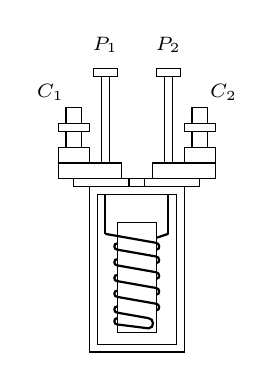
\begin{tikzpicture}
      % Inner core
      \draw (-0.25,0.15) rectangle (0.25,-1.25);
      % Window cut
      \draw (-0.5,0.5) rectangle (0.5,-1.4);
      % Outer wall
      \draw (-0.6,0.6) rectangle (0.6,-1.5);
      % Upper box rectangle and detail
      \draw (-0.8,0.7) rectangle (0.8,0.6);
      \draw (-0.1,0.7) rectangle (0.1,0.6);
      % Left and right terminal rectangles
      \draw (-1,0.9) rectangle (-0.2,0.7);
      \draw (0.2,0.9) rectangle (1,0.7);
      \draw (-1,1.1) rectangle (-0.6,0.9);
      \draw (0.6,1.1) rectangle (1,0.9);
      % C terminals
      \draw (-0.9,1.6) rectangle (-0.7,1.1);
      \draw[fill=white] (-1,1.4) rectangle (-0.6,1.3);
      \draw (0.7,1.6) rectangle (0.9,1.1);
      \draw[fill=white] (1,1.4) rectangle (0.6,1.3);
      \node at (-1.1,1.8) {\scriptsize{$C_1$}};
      \node at (1.1,1.8) {\scriptsize{$C_2$}};
      % P terminals
      \draw (-0.45,2) rectangle (-0.35,0.9);
      \draw (0.45,2) rectangle (0.35,0.9);
      \draw (-0.55,2.1) rectangle (-0.25,2);
      \draw (0.55,2.1) rectangle (0.25,2);
      \node at (-0.4,2.4) {\scriptsize{$P_1$}};
      \node at (0.4,2.4) {\scriptsize{$P_2$}};
      % the resistance
      \draw[thick] (-0.4,0.5) -- (-0.4,0);
      \draw[thick] (0.4,0.5) -- (0.4,0);
      \draw[thick] (0.4,0) -- (0.25,-0.05);
      \draw[thick] (-0.4,0) -- +(-10:0.65)
        to [out=0,in=0,looseness=1.5] +(0.65,-0.2);

      \foreach \y in {-0.2,-0.4,-0.6,-0.8}{
        \draw[thick] (-0.25,{\y+0.08}) to [out=180,in=180,looseness=1.5]
          (-0.25,\y) -- +(-10:0.5)
          to [out=0,in=0,looseness=1.5] +(0.5,-0.17);
      }
      \draw[thick] (-0.25,{-1+0.08}) to [out=180,in=180,looseness=1.5]
        (-0.25,-1) -- +(-10:0.4)
        to [out=0,in=0,looseness=1.5] +(0.4,-0.2) -- (-0.25,-1.15) 
        to [out=180,in=180,looseness=1.5] (-0.25,-1.07);
    \end{tikzpicture}
    \caption{Esquema representativo de la resistencia patrón.}
  \end{subfigure}
  \hfill
  \begin{subfigure}[c]{0.48\textwidth}
    \centering
    \begin{circuitikz}[european]
      \draw (-2,0) node[above]{$C_1$} to[short,o-*] (-1.25,0) coordinate (A)
        to[R=$R_\text{pat}$] (1.25,0) coordinate(B) to[short,*-o] (2,0) node[above]{$C_2$};

        \draw (A) -- ++(0,1.5) node[ocirc,label=above:$P_1$]{};
        \draw (B) -- ++(0,1.5) node[ocirc,label=above:$P_2$]{};
    \end{circuitikz}
    \vspace{1.5cm}
    \caption{Diagrama de circuito.}
  \end{subfigure}
  \caption{La conexión de Kelvin.}
  \label{fig_res_kelvin}
\end{figure}


Al medir la tensión mediante un voltímetro de alta impedancia en los bornes \(P\), no circula corriente por estos contactos, eliminando virtualmente la caída de tensión en los contactos y aislando la medida de la resistencia del cableado. Mientras que en los bornes \(C\) se usan exclusivamente para conectar la resistencia patrón al circuito de medida.

\subsection{Materiales de construcción}

La estabilidad térmica es el desafío principal en la construcción de un patrón físico. Se busca que el coeficiente de temperatura (\(\alpha\)) sea lo más cercano a cero posible en el rango de operación. Para ello se emplean aleaciones específicas:

\begin{description}
    \item[Manganina:] Es la aleación por excelencia para patrones de alta precisión. Compuesta típicamente por 84\% cobre, 12\% manganeso y 4\% níquel. Posee una fuerza electromotriz térmica muy baja respecto al cobre (\qty{2}{\micro\volt\per\kelvin}), lo que evita errores por pares termoeléctricos en los bornes. Su curva de resistencia contra temperatura es parabólica, con un máximo estable alrededor de los \qty{25}{\degreeCelsius}.
    
    \item[Constantán:] Aleación de 55\% cobre y 45\% níquel. Aunque tiene un \(\alpha\) muy bajo, genera una f.e.m. térmica alta contra el cobre (\(\approx \qty{40}{\micro\volt\per\kelvin}\)). Por ello, se prefiere su uso en resistencias de potencia o calefacción y no tanto en patrones de precisión de corriente continua, es aceptable en corriente alterna.
\end{description}

Los patrones de alta jerarquía suelen sumergirse en baños de aceite termostáticos y poseen orificios centrales para la inserción de termómetros, garantizando que la temperatura de trabajo sea aquella en la que fueron calibrados. La corriente máxima admisible (\(I_{\text{max}}\)) está limitada por la capacidad de disipación de potencia (\(P\)) del aire o aceite:
\begin{equation}
    I_{\text{max}} = \sqrt{\frac{P_{\text{disipable}}}{R}}
\end{equation}

\subsection{Jerarquía y Trazabilidad}

La existencia de estos patrones físicos de alta estabilidad (como los resistores de cuatro terminales de Manganina) permite establecer una \emph{cadena de trazabilidad}.

Dado que la clase de un instrumento representa su error máximo permitido (ver definición en la sección \ref{sec_glosario}), para calibrar un instrumento de una determinada clase, se requiere siempre un patrón de una clase inferior (es decir, mayor exactitud).

Los Patrones Primarios y Secundarios (resistores de 4 bornes) poseen las clases más bajas (ej. 0.001) y se utilizan para calibrar a los instrumentos de laboratorio de alta precisión. Estos instrumentos de alta precisión actúan luego como Patrones de Trabajo para calibrar a los instrumentos de uso industrial o de campo (clases 1.0, 1.5, etc.), donde los errores de conexión (como la resistencia de los cables) son despreciables frente al error propio del instrumento.

De esta forma, la exactitud se ``transfiere'' desde las definiciones fundamentales del SI hasta el instrumento del operario, degradándose controladamente en cada escalón, pero manteniendo siempre una referencia conocida.

\subsection{Comportamiento en Corriente Alterna: La Impedancia}

Cuando la f.e.m (\(\mathcal{E}\)) que produce la diferencia de potencial genera una señal en función del tiempo (\(v(t)\)), se obtiene una corriente alterna (ca). Este hecho implica que el comportamiento en algunos componentes como inductores y capacitores cambie con respecto a la corriente continua. Para continuar con este apartado es ideal tener una noción básica sobre electrotecnia y análisis de circuitos, el libro \citetitle{electrotecnia_matthew} de \textcite{electrotecnia_matthew} contiene una guía elemental y muy detallada sobre estos conceptos.

Un resistor ideal se comporta de manera idéntica tanto en corriente continua como en alterna, obedeciendo la Ley de Ohm en todo instante. Si definimos una corriente sinusoidal \(i(t) = I_{\text{max}} \sin(\omega t)\), la tensión en los bornes será:
\begin{equation}
    u_R(t) = R \cdot i(t) = R \cdot I_{\text{max}} \sin(\omega t)
\end{equation}
Como se observa, la tensión y la corriente están perfectamente en fase (\(\omega\)).

Sin embargo, los resistores reales poseen características físicas inevitables que alteran este comportamiento: la geometría del alambre genera una autoinducción (\(L\)) y la proximidad entre espiras crea una capacidad parásita (\(C\)). Recordando las definiciones vistas en la sección \ref{sec_unidades} de unidades:
\begin{itemize}
  \item \textbf{Inductancia (\(L\)):} Se opone a las variaciones de corriente generando una tensión proporcional a su derivada.
  \[ u_L(t) = L \frac{di(t)}{dt} = L \cdot \omega I_{\text{max}} \cos(\omega t) \]
  Esto adelanta la tensión \(90^\circ\) respecto a la corriente.
  
  \item \textbf{Capacitancia (\(C\)):} Se opone a las variaciones de tensión, donde la corriente es proporcional a la derivada de la tensión.
  \[ i_C(t) = C \frac{du(t)}{dt} \]
  Esto provoca un efecto inverso, retrasando la tensión respecto a la corriente.
\end{itemize}

Resolver este comportamiento mediante ecuaciones diferenciales en el tiempo resulta tedioso. Para simplificar el análisis en régimen permanente sinusoidal, recurrimos al concepto de Impedancia Compleja (\(\mathbf{Z}\)) utilizando fasores. La impedancia generaliza la resistencia, permitiendo sumar los efectos resistivos y reactivos algebraicamente:
\[
  \mathbf{Z} = R + jX
\]
Donde \(R\) es la parte resistiva y \(X\) la reactancia. Modelando el resistor real como un circuito serie R-L-C simplificado\footnote{A modo de repaso sobre circuitos RLC, puede mirar los siguientes recursos multimedia: \url{https://youtu.be/sho9Qqr4-Gs?si=rl2uFHjTuxpGjOqL} y \url{https://youtu.be/HonwOVt0zvo?si=robFXBs4e_bqu0J9}}, la impedancia total es:
\begin{equation}\label{eq:impedancia_compleja}
  \mathbf{Z} = R + j\omega L + \frac{1}{j\omega C} = R + j\left(\omega L - \frac{1}{\omega C}\right)
\end{equation}

El valor que finalmente limita la corriente o define la caída de tensión es el módulo de esta impedancia:
\begin{equation}
  |\mathbf{Z}| = \sqrt{R^2 + \left(\omega L - \frac{1}{\omega C}\right)^2}
\end{equation}

Para que un resistor patrón sea confiable en corriente alterna, su impedancia \(\mathbf{Z}\) debe ser lo más parecida posible a su resistencia en corriente continua \(R\). Observando la ecuación \eqref{eq:impedancia_compleja}, esto implica que el término imaginario (reactancia) debe ser, idealmente, nulo:
\[ \omega L - \frac{1}{\omega C} \approx 0 \]
Dado que la frecuencia \(\omega\) es una variable externa que no controlamos, el fabricante debe garantizar mediante el diseño constructivo que tanto \(L\) (inductancia) como \(C\) (capacitancia) tiendan a cero.

Para lograr la anulación de los componentes reactivos descritos anteriormente, se emplean técnicas de bobinado especiales que cancelan los campos magnéticos y eléctricos:

\begin{enumerate}
  \item \textbf{Bobinado Bifilar (Ayrton-Perry):} El alambre se pliega por la mitad antes de arrollarse sobre el núcleo. De esta forma, dos corrientes de igual magnitud circulan en direcciones opuestas (\(\vec{I}\) y \(-\vec{I}\)) por conductores adyacentes. El efecto en \(L\) es que los flujos magnéticos generados por cada mitad del alambre se oponen entre sí, cancelándose mutuamente y reduciendo la autoinducción a valores despreciables.
  
  \item \textbf{Bobinado Plano (Tarjeta o Rowland):} Se utiliza principalmente para reducir la capacidad parásita en resistencias de alto valor. El hilo se enrolla en una tarjeta plana aislante de forma delgada. El efecto en \(C\) es que al disponer el alambre de forma plana, se reduce la superficie enfrentada entre espiras con gran diferencia de potencial, minimizando así el efecto de capacitor de placas paralelas distribuidas.
\end{enumerate}
